\documentclass{article}
\usepackage[margin=1in]{geometry}
\usepackage{datetime}
\usepackage{qcircuit}
\usepackage{amsmath}
\usepackage{pgfplots}
\pgfplotsset{compat=1.18}
\usepackage[utf8]{inputenc}
\begin{document}
\noindent
\text{mimiQ++ report - \today\ \currenttime} 

\clearpage
\begin{figure}[htbp]
\[
\Qcircuit @C=1em @R=.7em {
\lstick{q0} & \gate{U(0.3,0.2,0.1)} & \qw & \ctrl{1} & \gate{H} & \meter & \qw & \qw & \qw & \qw & \qw & \\ 
\lstick{q1} & \gate{H} & \ctrl{1} & \gate{X} & \qw & \qw \cwx & \meter & \qw & \qw & \qw & \qw & \\ 
\lstick{q2} & \qw & \gate{X} & \qw & \qw & \qw \cwx & \qw \cwx & \gate{X} & \gate{Z} & \meter & \qw & \\ 
\lstick{c0} & \cw & \cw & \cw & \cw & \cw \cwx & \cw \cwx & \cw \cwx & \control \cw \cwx & \cw \cwx & \cw & \\ 
\lstick{c1} & \cw & \cw & \cw & \cw & \cw & \cw \cwx & \control \cw \cwx & \cw & \cw \cwx & \cw & \\ 
\lstick{c2} & \cw & \cw & \cw & \cw & \cw & \cw & \cw & \cw & \cw \cwx & \cw & \\ 
\\ 
\\ 
}
\]
\caption{quantum teleportation 1}
\end{figure}






\text{Classical register readings (left to right: cn,cn-1,..c2,c1,c0) for the simulation:} 





000: 246


100: 5


010: 246


110: 11


001: 261


101: 6


011: 241


111: 8


\begin{center}
    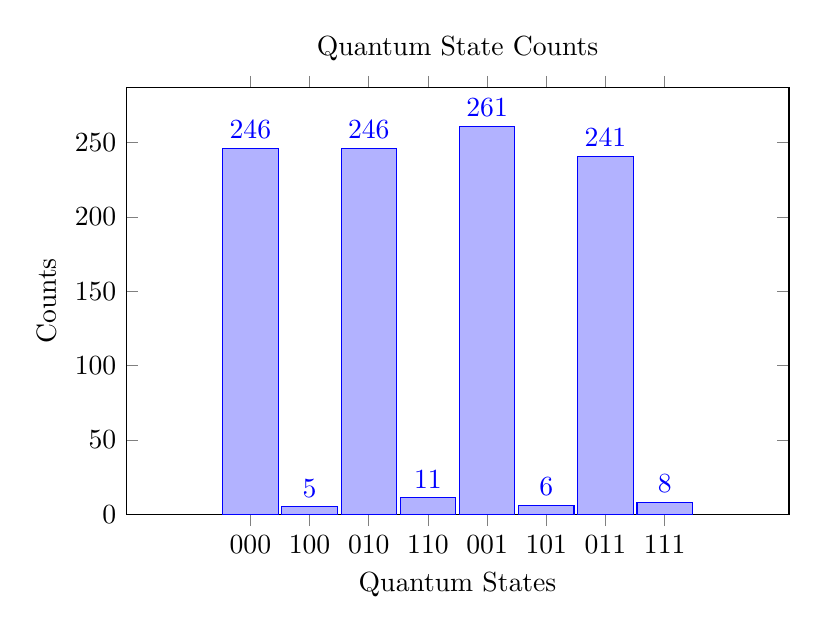
\begin{tikzpicture}
        \begin{axis}[
            ybar,
            symbolic x coords={000, 100, 010, 110, 001, 101, 011, 111},
            xtick=data,
            xlabel={Quantum States},
            ylabel={Counts},
            ymin=0,
            bar width=20pt,
            width=10cm,
            height=7cm,
            nodes near coords,
            nodes near coords align={vertical},
            enlarge x limits=0.3,
            title={Quantum State Counts}
        ]
        \addplot coordinates {(000,246) (100,5) (010,246) (110,11) (001,261) (101,6) (011,241) (111,8) };
        \end{axis}
    \end{tikzpicture}
\end{center}


\clearpage
\begin{figure}[htbp]
\[
\Qcircuit @C=1em @R=.7em {
\lstick{q0} & \gate{U(6.28,0.408,2.22)} & \qw & \ctrl{1} & \gate{H} & \meter & \qw & \qw & \qw &  \qw & \\
\lstick{q1} & \gate{H} & \ctrl{1} & \gate{X} & \qw & \qw \cwx & \meter & \qw & \qw &  \qw & \\
\lstick{q2} & \qw & \gate{X} & \qw & \qw & \qw \cwx & \qw \cwx & \gate{X} & \gate{Z} &  \qw & \\
\lstick{c0} & \cw & \cw & \cw & \cw & \cw \cwx & \cw \cwx & \cw \cwx & \control \cw \cwx &  \cw & \\
\lstick{c1} & \cw & \cw & \cw & \cw & \cw & \cw \cwx & \control \cw \cwx & \cw &  \cw & \\
\lstick{c2} & \cw & \cw & \cw & \cw & \cw & \cw & \cw & \cw &  \cw & \\
\\ 
\\ 
\lstick{q0} & \qw & \qw & \qw & \\ 
\lstick{q1} & \qw & \qw & \qw & \\ 
\lstick{q2} & \gate{U(-6.28,-2.22,-0.408)} & \meter & \qw & \\ 
\lstick{c0} & \cw & \cw \cwx & \cw & \\ 
\lstick{c1} & \cw & \cw \cwx & \cw & \\ 
\lstick{c2} & \cw & \cw \cwx & \cw & \\ 
\\ 
\\ 
}
\]
\caption{quantum teleportation ibm}
\end{figure}






\text{Classical register readings (left to right: cn,cn-1,..c2,c1,c0) for the simulation:} 





000: 254


010: 259


001: 240


011: 271


\begin{center}
    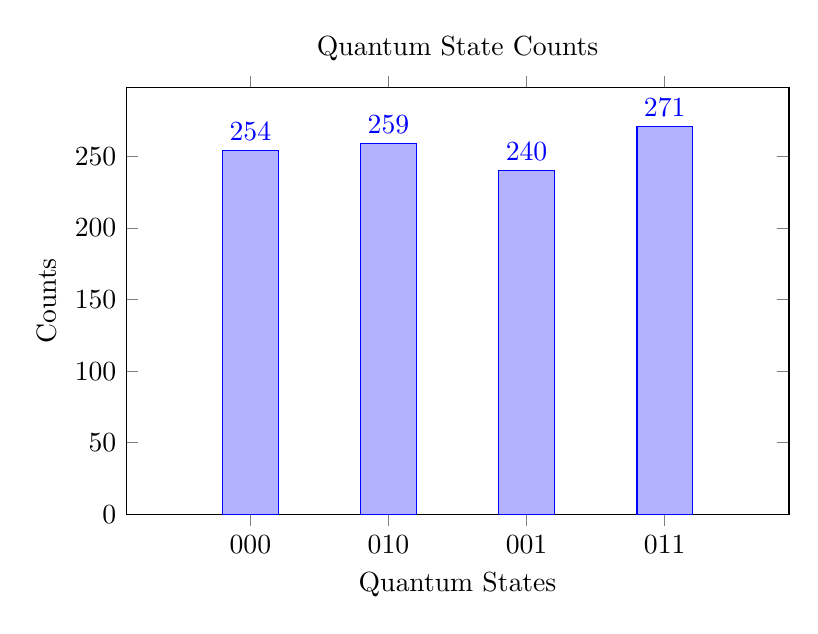
\begin{tikzpicture}
        \begin{axis}[
            ybar,
            symbolic x coords={000, 010, 001, 011},
            xtick=data,
            xlabel={Quantum States},
            ylabel={Counts},
            ymin=0,
            bar width=20pt,
            width=10cm,
            height=7cm,
            nodes near coords,
            nodes near coords align={vertical},
            enlarge x limits=0.3,
            title={Quantum State Counts}
        ]
        \addplot coordinates {(000,254) (010,259) (001,240) (011,271) };
        \end{axis}
    \end{tikzpicture}
\end{center}


\clearpage
\begin{figure}[htbp]
\[
\Qcircuit @C=1em @R=.7em {
\lstick{q0} & \gate{X} & \meter & \gate{X} & \gate{H} & \ctrl{1} & \gate{Z} & \gate{X} & \ctrl{1} & \gate{H} & \meter & \qw & \qw & \\ 
\lstick{q1} & \qw & \qw \cwx & \qw & \qw & \gate{X} & \qw \cwx & \qw \cwx & \gate{X} & \qw & \qw \cwx & \meter & \qw & \\ 
\lstick{c0} & \cw & \cw \cwx & \cw & \cw & \cw & \cw \cwx & \control \cw \cwx & \cw & \cw & \cw \cwx & \cw \cwx & \cw & \\ 
\lstick{c1} & \cw & \cw \cwx & \cw & \cw & \cw & \control \cw \cwx & \cw & \cw & \cw & \cw \cwx & \cw \cwx & \cw & \\ 
\lstick{c2} & \cw & \cw & \cw & \cw & \cw & \cw & \cw & \cw & \cw & \cw \cwx & \cw \cwx & \cw & \\ 
\lstick{c3} & \cw & \cw & \cw & \cw & \cw & \cw & \cw & \cw & \cw & \cw \cwx & \cw & \cw & \\ 
\\ 
\\ 
}
\]
\caption{superdense coding}
\end{figure}






\text{Classical register readings (left to right: cn,cn-1,..c2,c1,c0) for the simulation:} 





1010: 1024


\begin{center}
    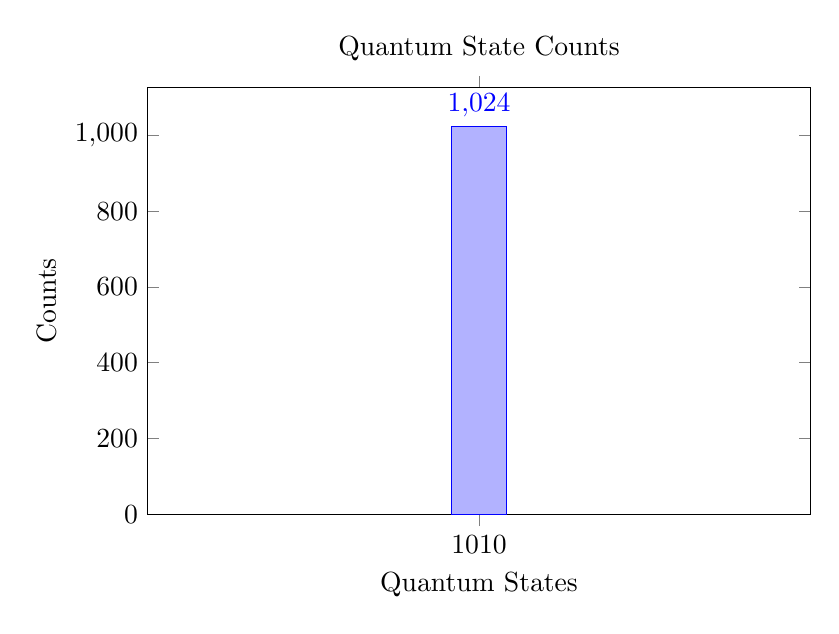
\begin{tikzpicture}
        \begin{axis}[
            ybar,
            symbolic x coords={1010},
            xtick=data,
            xlabel={Quantum States},
            ylabel={Counts},
            ymin=0,
            bar width=20pt,
            width=10cm,
            height=7cm,
            nodes near coords,
            nodes near coords align={vertical},
            enlarge x limits=0.3,
            title={Quantum State Counts}
        ]
        \addplot coordinates {(1010,1024) };
        \end{axis}
    \end{tikzpicture}
\end{center}


\clearpage
\begin{figure}[htbp]
\[
\Qcircuit @C=1em @R=.7em {
\lstick{q0} & \gate{H} & \qw & \qw & \qw & \qw & \ctrl{1} & \gate{Z} & \gate{X} & \ctrl{1} & \gate{H} & \meter & \qw & \qw & \\ 
\lstick{q1} & \qw & \qw & \qw & \qw & \qw & \gate{X} & \qw \cwx & \qw \cwx & \gate{X} & \qw & \qw \cwx & \meter & \qw & \\ 
\lstick{q2} & \gate{H} & \meter & \gate{X} & \gate{H} & \meter & \qw & \qw \cwx & \qw \cwx & \qw & \qw & \qw \cwx & \qw \cwx & \qw & \\ 
\lstick{c0} & \cw & \cw \cwx & \control \cw \cwx & \cw & \cw \cwx & \cw & \cw \cwx & \control \cw \cwx & \cw & \cw & \cw \cwx & \cw \cwx & \cw & \\ 
\lstick{c1} & \cw & \cw & \cw & \cw & \cw \cwx & \cw & \control \cw \cwx & \cw & \cw & \cw & \cw \cwx & \cw \cwx & \cw & \\ 
\lstick{c2} & \cw & \cw & \cw & \cw & \cw & \cw & \cw & \cw & \cw & \cw & \cw \cwx & \cw \cwx & \cw & \\ 
\lstick{c3} & \cw & \cw & \cw & \cw & \cw & \cw & \cw & \cw & \cw & \cw & \cw \cwx & \cw & \cw & \\ 
\\ 
\\ 
}
\]
\caption{superdense coding - random}
\end{figure}






\text{Classical register readings (left to right: cn,cn-1,..c2,c1,c0) for the simulation:} 





0000: 256


1010: 258


0101: 241


1111: 269


\begin{center}
    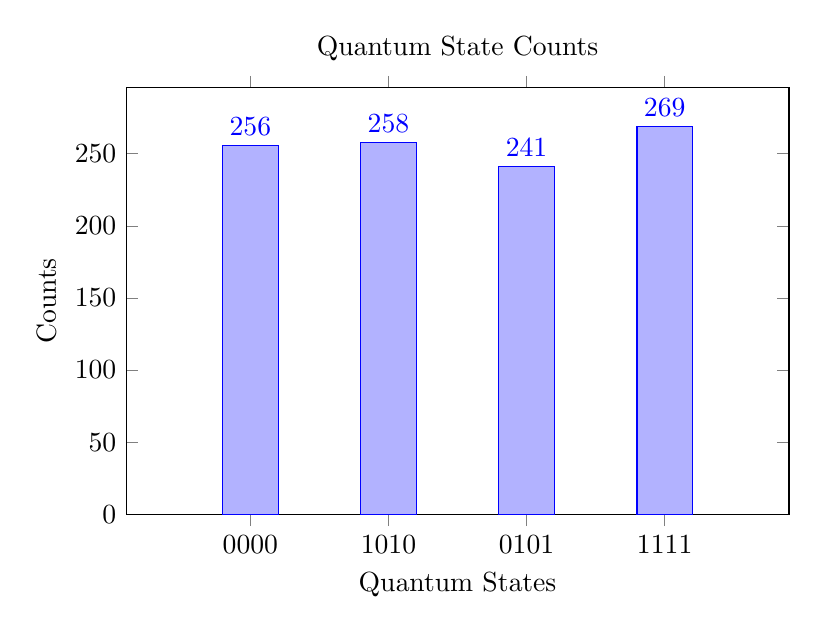
\begin{tikzpicture}
        \begin{axis}[
            ybar,
            symbolic x coords={0000, 1010, 0101, 1111},
            xtick=data,
            xlabel={Quantum States},
            ylabel={Counts},
            ymin=0,
            bar width=20pt,
            width=10cm,
            height=7cm,
            nodes near coords,
            nodes near coords align={vertical},
            enlarge x limits=0.3,
            title={Quantum State Counts}
        ]
        \addplot coordinates {(0000,256) (1010,258) (0101,241) (1111,269) };
        \end{axis}
    \end{tikzpicture}
\end{center}


\clearpage
\begin{figure}[htbp]
\[
\Qcircuit @C=1em @R=.7em {
\lstick{q0} & \qw & \qw & \qw & \gate{X} & \qw & \qw & \qw & \gate{H} & \qw & \qw & \qw & \qw & \qw & \meter &  \qw & \\
\lstick{q1} & \gate{H} & \meter & \gate{X} & \qw \cwx & \gate{H} & \meter & \gate{X} & \qw \cwx & \gate{H} & \meter & \gate{X} & \gate{H} & \meter & \qw \cwx &  \qw & \\
\lstick{c0} & \cw & \cw \cwx & \control \cw \cwx & \control \cw \cwx & \cw & \cw \cwx & \cw \cwx & \cw \cwx & \cw & \cw \cwx & \cw \cwx & \cw & \cw \cwx & \cw \cwx &  \cw & \\
\lstick{c1} & \cw & \cw & \cw & \cw & \cw & \cw \cwx & \control \cw \cwx & \control \cw \cwx & \cw & \cw \cwx & \cw \cwx & \cw & \cw \cwx & \cw \cwx &  \cw & \\
\lstick{c2} & \cw & \cw & \cw & \cw & \cw & \cw & \cw & \cw & \cw & \cw \cwx & \cw \cwx & \cw & \cw \cwx & \cw \cwx &  \cw & \\
\lstick{c3} & \cw & \cw & \cw & \cw & \cw & \cw & \cw & \cw & \cw & \cw \cwx & \cw \cwx & \cw & \cw & \cw \cwx &  \cw & \\
\lstick{c4} & \cw & \cw & \cw & \cw & \cw & \cw & \cw & \cw & \cw & \cw \cwx & \control \cw \cwx & \cw & \cw & \cw &  \cw & \\
\lstick{c5} & \cw & \cw & \cw & \cw & \cw & \cw & \cw & \cw & \cw & \cw & \cw & \cw & \cw & \cw &  \cw & \\
\\ 
\\ 
\lstick{q0} & \qw & \\ 
\lstick{q1} & \qw & \\ 
\lstick{c0} & \cw & \\ 
\lstick{c1} & \cw & \\ 
\lstick{c2} & \cw & \\ 
\lstick{c3} & \cw & \\ 
\lstick{c4} & \cw & \\ 
\lstick{c5} & \cw & \\ 
\\ 
\\ 
}
\]
\caption{BB98-ptcl QKD}
\end{figure}
Resultant key: 01101101111101111100001011011011011101111100000111

\clearpage
\begin{figure}[htbp]
\[
\Qcircuit @C=1em @R=.7em {
\lstick{q0} & \gate{H} & \gate{X} & \ctrl{2} & \gate{X} & \gate{H} & \gate{X} & \qw & \ctrl{2} & \gate{X} & \gate{H} & \gate{X} & \qw & \ctrl{2} & \gate{X} &  \qw & \\
\lstick{q1} & \gate{H} & \qw & \ctrl{1} & \gate{H} & \gate{X} & \qw & \qw & \ctrl{1} & \gate{X} & \gate{H} & \qw & \qw & \ctrl{1} & \gate{H} &  \qw & \\
\lstick{q2} & \gate{H} & \gate{H} & \gate{X} & \gate{H} & \gate{H} & \gate{X} & \gate{H} & \gate{X} & \gate{H} & \gate{X} & \gate{H} & \gate{H} & \gate{X} & \gate{H} &  \qw & \\
\lstick{c0} & \cw & \cw & \cw & \cw & \cw & \cw & \cw & \cw & \cw & \cw & \cw & \cw & \cw & \cw &  \cw & \\
\lstick{c1} & \cw & \cw & \cw & \cw & \cw & \cw & \cw & \cw & \cw & \cw & \cw & \cw & \cw & \cw &  \cw & \\
\lstick{c2} & \cw & \cw & \cw & \cw & \cw & \cw & \cw & \cw & \cw & \cw & \cw & \cw & \cw & \cw &  \cw & \\
\\ 
\\ 
\lstick{q0} & \gate{H} & \gate{X} & \qw & \ctrl{2} & \gate{X} & \gate{H} & \qw & \meter & \qw & \qw & \qw & \\ 
\lstick{q1} & \gate{X} & \qw & \qw & \ctrl{1} & \gate{X} & \gate{H} & \qw & \qw \cwx & \meter & \qw & \qw & \\ 
\lstick{q2} & \gate{H} & \gate{X} & \gate{H} & \gate{X} & \gate{H} & \gate{X} & \gate{H} & \qw \cwx & \qw \cwx & \meter & \qw & \\ 
\lstick{c0} & \cw & \cw & \cw & \cw & \cw & \cw & \cw & \cw \cwx & \cw \cwx & \cw \cwx & \cw & \\ 
\lstick{c1} & \cw & \cw & \cw & \cw & \cw & \cw & \cw & \cw & \cw \cwx & \cw \cwx & \cw & \\ 
\lstick{c2} & \cw & \cw & \cw & \cw & \cw & \cw & \cw & \cw & \cw & \cw \cwx & \cw & \\ 
\\ 
\\ 
}
\]
\caption{grover}
\end{figure}






\text{Classical register readings (left to right: cn,cn-1,..c2,c1,c0) for the simulation:} 





000: 5


100: 5


010: 7


110: 945


001: 6


101: 12


011: 7


111: 13


\begin{center}
    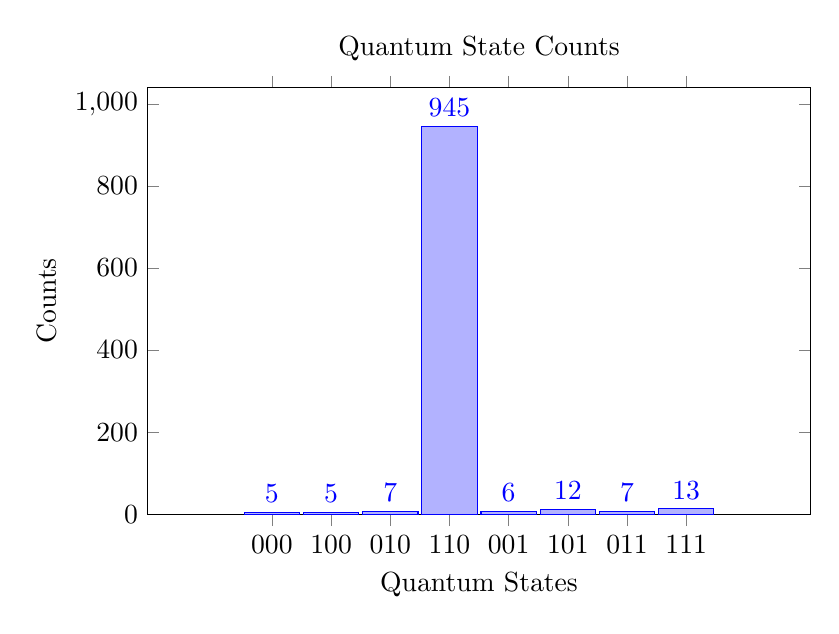
\begin{tikzpicture}
        \begin{axis}[
            ybar,
            symbolic x coords={000, 100, 010, 110, 001, 101, 011, 111},
            xtick=data,
            xlabel={Quantum States},
            ylabel={Counts},
            ymin=0,
            bar width=20pt,
            width=10cm,
            height=7cm,
            nodes near coords,
            nodes near coords align={vertical},
            enlarge x limits=0.3,
            title={Quantum State Counts}
        ]
        \addplot coordinates {(000,5) (100,5) (010,7) (110,945) (001,6) (101,12) (011,7) (111,13) };
        \end{axis}
    \end{tikzpicture}
\end{center}


\clearpage
\begin{figure}[htbp]
\[
\Qcircuit @C=1em @R=.7em {
\lstick{q0} & \gate{X} & \ctrl{2} & \ctrl{1} & \qw & \qw & \ctrl{1} & \meter & \qw & \qw & \qw & \qw & \\ 
\lstick{q1} & \qw & \ctrl{1} & \gate{X} & \ctrl{2} & \ctrl{1} & \gate{X} & \qw \cwx & \meter & \qw & \qw & \qw & \\ 
\lstick{q2} & \gate{X} & \gate{X} & \qw & \ctrl{1} & \gate{X} & \qw & \qw \cwx & \qw \cwx & \meter & \qw & \qw & \\ 
\lstick{q3} & \qw & \qw & \qw & \gate{X} & \qw & \qw & \qw \cwx & \qw \cwx & \qw \cwx & \meter & \qw & \\ 
\lstick{c0} & \cw & \cw & \cw & \cw & \cw & \cw & \cw \cwx & \cw \cwx & \cw \cwx & \cw \cwx & \cw & \\ 
\lstick{c1} & \cw & \cw & \cw & \cw & \cw & \cw & \cw & \cw \cwx & \cw \cwx & \cw \cwx & \cw & \\ 
\lstick{c2} & \cw & \cw & \cw & \cw & \cw & \cw & \cw & \cw & \cw \cwx & \cw \cwx & \cw & \\ 
\lstick{c3} & \cw & \cw & \cw & \cw & \cw & \cw & \cw & \cw & \cw & \cw \cwx & \cw & \\ 
\\ 
\\ 
}
\]
\caption{full adder}
\end{figure}






\text{Classical register readings (left to right: cn,cn-1,..c2,c1,c0) for the simulation:} 





1001: 1000


\begin{center}
    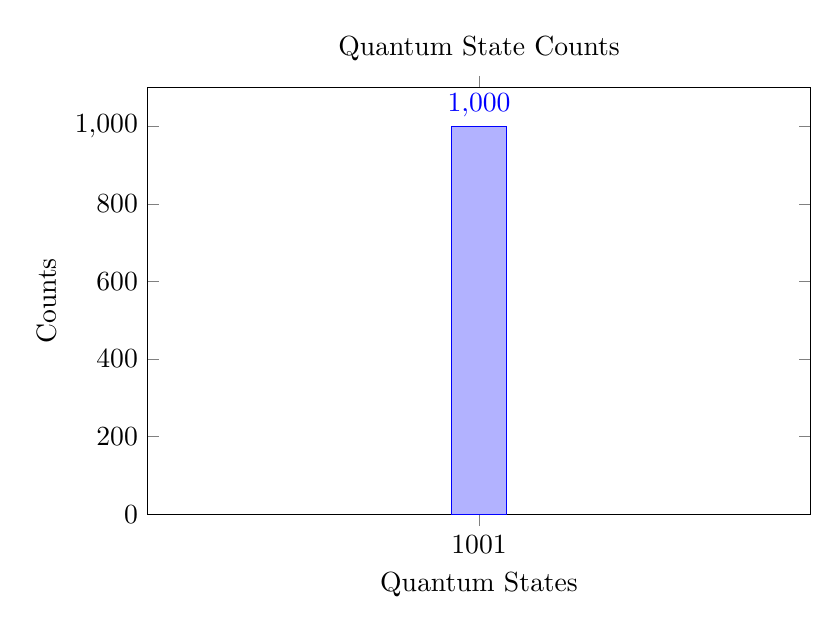
\begin{tikzpicture}
        \begin{axis}[
            ybar,
            symbolic x coords={1001},
            xtick=data,
            xlabel={Quantum States},
            ylabel={Counts},
            ymin=0,
            bar width=20pt,
            width=10cm,
            height=7cm,
            nodes near coords,
            nodes near coords align={vertical},
            enlarge x limits=0.3,
            title={Quantum State Counts}
        ]
        \addplot coordinates {(1001,1000) };
        \end{axis}
    \end{tikzpicture}
\end{center}


\clearpage
\begin{figure}[htbp]
\[
\Qcircuit @C=1em @R=.7em {
\lstick{q0} & \gate{H} & \qw & \qw & \qw & \qw & \ctrl{2} & \ctrl{2} & \qw & \ctrl{2} & \qw &  \qw & \\
\lstick{q1} & \gate{H} & \ctrl{1} & \qw & \ctrl{1} & \gate{X} & \ctrl{1} & \qw & \qw & \qw & \qw &  \qw & \\
\lstick{q2} & \qw & \gate{X} & \gate{Ry(0.111)} & \gate{X} & \gate{Ry(-0.111)} & \gate{X} & \gate{X} & \gate{Ry(0)} & \gate{X} & \gate{Ry(0)} &  \qw & \\
\lstick{q3} & \qw & \qw & \qw & \qw & \qw & \qw & \qw & \qw & \qw & \qw &  \qw & \\
\lstick{c0} & \cw & \cw & \cw & \cw & \cw & \cw & \cw & \cw & \cw & \cw &  \cw & \\
\lstick{c1} & \cw & \cw & \cw & \cw & \cw & \cw & \cw & \cw & \cw & \cw &  \cw & \\
\lstick{c2} & \cw & \cw & \cw & \cw & \cw & \cw & \cw & \cw & \cw & \cw &  \cw & \\
\lstick{c3} & \cw & \cw & \cw & \cw & \cw & \cw & \cw & \cw & \cw & \cw &  \cw & \\
\\ 
\\ 
\lstick{q0} & \ctrl{2} & \ctrl{2} & \qw & \ctrl{2} & \gate{X} & \ctrl{2} & \ctrl{2} & \qw & \ctrl{2} & \qw & \ctrl{2} &  \qw & \\
\lstick{q1} & \ctrl{1} & \qw & \qw & \qw & \qw & \ctrl{1} & \qw & \qw & \qw & \qw & \ctrl{1} &  \qw & \\
\lstick{q2} & \gate{X} & \gate{X} & \gate{Ry(0)} & \gate{X} & \gate{Ry(0)} & \gate{X} & \gate{X} & \gate{Ry(-1.511)} & \gate{X} & \gate{Ry(1.511)} & \gate{X} &  \qw & \\
\lstick{q3} & \qw & \qw & \qw & \qw & \qw & \qw & \qw & \qw & \qw & \qw & \qw &  \qw & \\
\lstick{c0} & \cw & \cw & \cw & \cw & \cw & \cw & \cw & \cw & \cw & \cw & \cw &  \cw & \\
\lstick{c1} & \cw & \cw & \cw & \cw & \cw & \cw & \cw & \cw & \cw & \cw & \cw &  \cw & \\
\lstick{c2} & \cw & \cw & \cw & \cw & \cw & \cw & \cw & \cw & \cw & \cw & \cw &  \cw & \\
\lstick{c3} & \cw & \cw & \cw & \cw & \cw & \cw & \cw & \cw & \cw & \cw & \cw &  \cw & \\
\\ 
\\ 
\lstick{q0} & \ctrl{2} & \qw & \ctrl{2} & \qw & \ctrl{3} & \qw & \qw & \qw & \qw & \\ 
\lstick{q1} & \qw & \qw & \qw & \qw & \qw & \gate{H} & \meter & \qw & \qw & \\ 
\lstick{q2} & \gate{X} & \gate{Ry(1.511)} & \gate{X} & \gate{Ry(-1.511)} & \qw & \qw & \qw \cwx & \qw & \qw & \\ 
\lstick{q3} & \qw & \qw & \qw & \qw & \gate{X} & \qw & \qw \cwx & \meter & \qw & \\ 
\lstick{c0} & \cw & \cw & \cw & \cw & \cw & \cw & \cw \cwx & \cw \cwx & \cw & \\ 
\lstick{c1} & \cw & \cw & \cw & \cw & \cw & \cw & \cw \cwx & \cw \cwx & \cw & \\ 
\lstick{c2} & \cw & \cw & \cw & \cw & \cw & \cw & \cw & \cw \cwx & \cw & \\ 
\lstick{c3} & \cw & \cw & \cw & \cw & \cw & \cw & \cw & \cw \cwx & \cw & \\ 
\\ 
\\ 
}
\]
\caption{quantum classification}
\end{figure}






\text{Classical register readings (left to right: cn,cn-1,..c2,c1,c0) for the simulation:} 





0000: 508


1000: 10


1010: 482


\begin{center}
    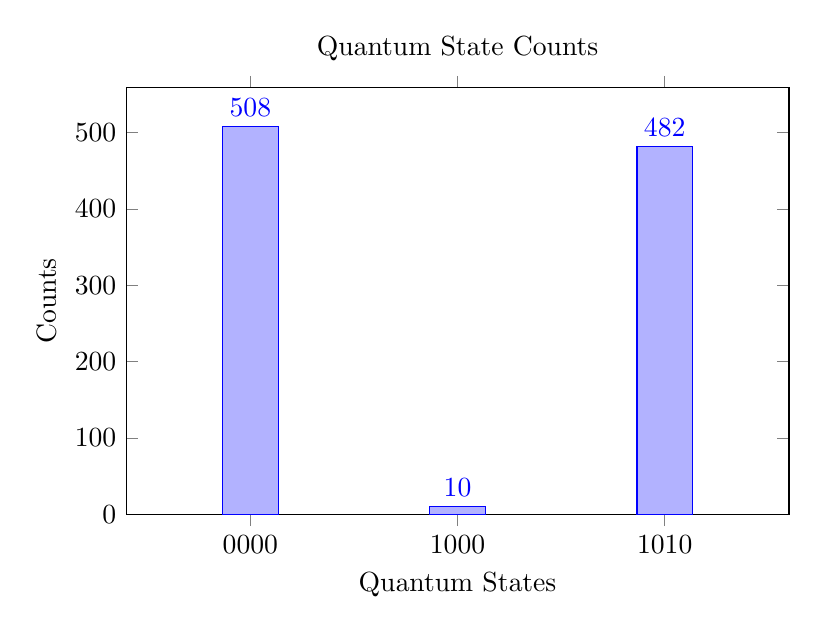
\begin{tikzpicture}
        \begin{axis}[
            ybar,
            symbolic x coords={0000, 1000, 1010},
            xtick=data,
            xlabel={Quantum States},
            ylabel={Counts},
            ymin=0,
            bar width=20pt,
            width=10cm,
            height=7cm,
            nodes near coords,
            nodes near coords align={vertical},
            enlarge x limits=0.3,
            title={Quantum State Counts}
        ]
        \addplot coordinates {(0000,508) (1000,10) (1010,482) };
        \end{axis}
    \end{tikzpicture}
\end{center}


\end{document}